\documentclass{article}

\usepackage{graphicx}
\usepackage{tikz}
\usepackage{tikzsymbols}
\usetikzlibrary{calc,patterns,shapes.geometric}
\pagestyle{empty}
\usepackage[margin=0pt]{geometry}
\geometry{papersize={14in,12in}}

\def\centerarc[#1](#2)(#3:#4:#5){\draw[#1] ($(#2)+({#5*cos(#3)},{#5*sin(#3)})$) arc (#3:#4:#5);}

\begin{document}
	\begin{figure}
		\centering
		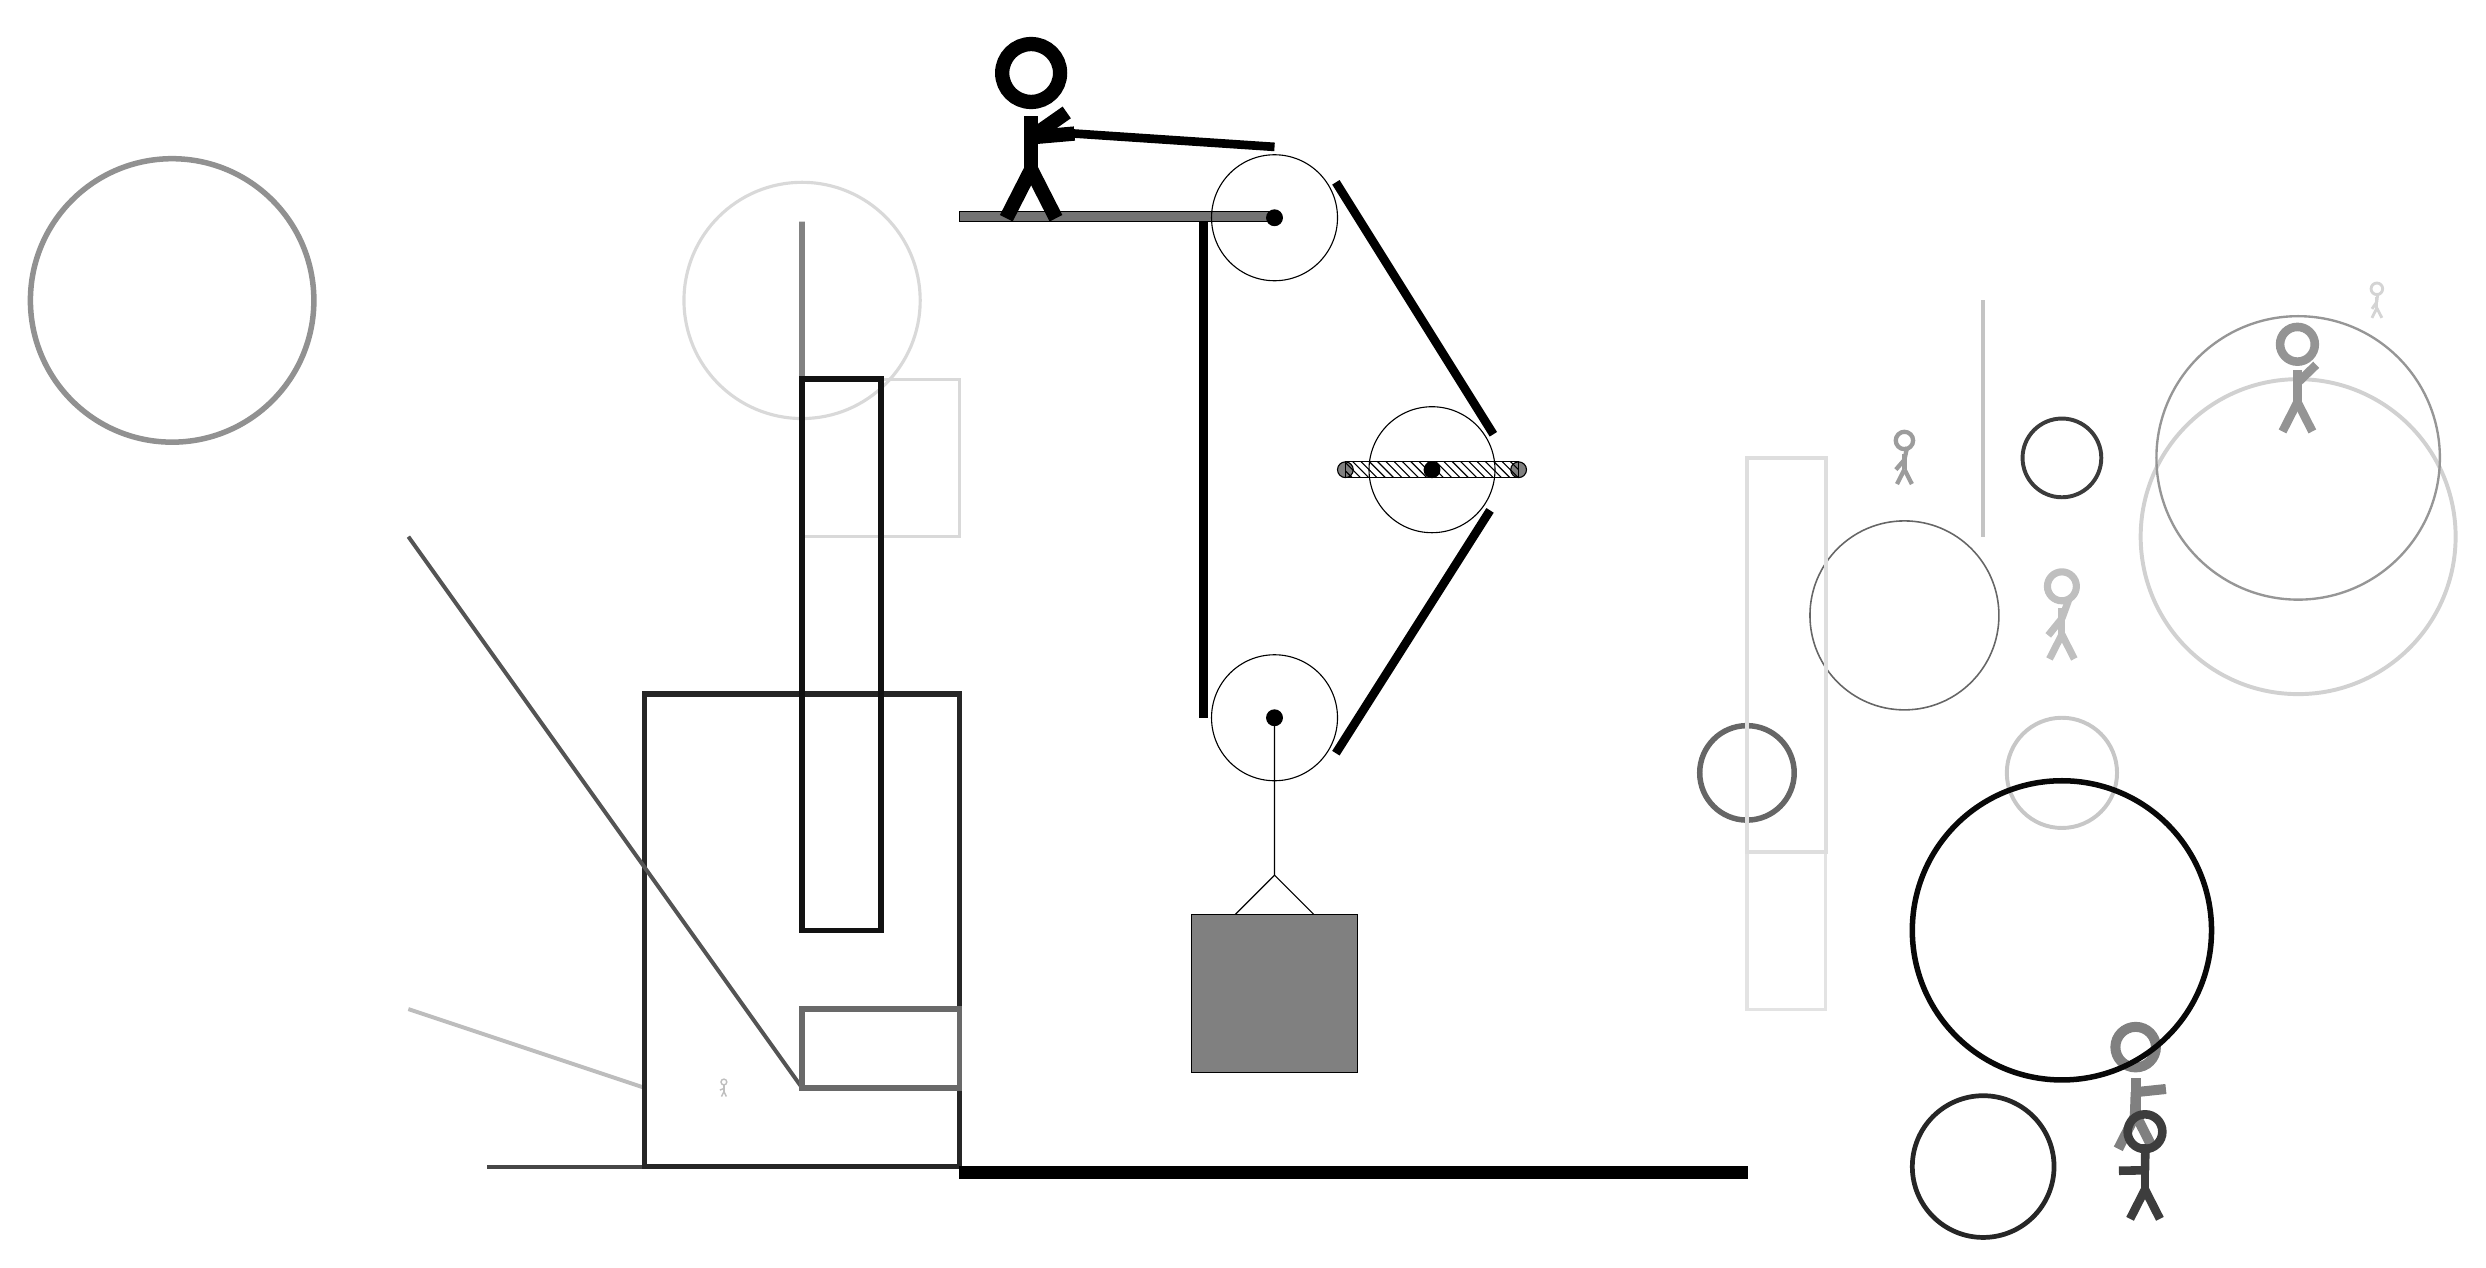
\begin{tikzpicture}
			%%%%% START %%%%%
			
			\draw[fill=black!55] (-2, 9) rectangle (2, 9.125);
			
			\draw (2, 2.7) circle (0.8);
			\draw[fill=black] (2, 2.7) circle (0.1);
			
			\draw (2, 9.05) circle (0.8);
			\draw[fill=black] (2, 9.05) circle (0.1);
			
			\draw[fill=white](4, 5.85) circle (0.8);
			\draw[fill=black] (4, 5.85) circle (0.1);
			\draw[fill=black!50] (2.9, 5.85) circle (0.1);
			\draw[fill=black!50] (5.1, 5.85) circle (0.1);
			\draw[pattern=north west lines, pattern color=black] (2.9, 5.95) rectangle (5.1, 5.75);
			
			\draw (2, 2.7) -- (2, 0.7) -- (1.5, 0.2) -- (2.5, 0.2) -- (2, 0.7);
			\draw[fill=black!50] (0.95, 0.2) rectangle (3.05, -1.8);
			
			\node[line width=0.2mm, color=black!39] at (10, 6) {\Strichmaxerl[3][49][78]};
			
			\draw[line width=0.4mm, color=black!15] (-2, 7) rectangle (-4, 5);
			\node[line width=0.4mm, color=black!50] at (13, -2) {\Strichmaxerl[7][88][6]};
			\node[line width=0.7mm, color=black!76] at (13, -3) {\Strichmaxerl[6][1][89]};
			
			\draw[line width=0.4mm, color=black!11] (9, 6) rectangle (8, -1);
			\draw [line width=0.5mm, color=black!18](15, 5) circle (2.0);
			\node[line width=0.5mm, color=black!25] at (12, 4) {\Strichmaxerl[5][51][70]};
			\node[line width=0.3mm, color=black!17] at (16, 8) {\Strichmaxerl[2][56][84]};
			\draw [line width=0.5mm, color=black!77](12, 6) circle (0.5);
			
			\draw [line width=0.2mm, color=black!60](10, 4) circle (1.2);
			\draw[line width=0.7mm, color=black!49] (-4, 1) rectangle (-4, 9);
			
			\draw[line width=0.5mm, color=black!72](-3, -3) -- (-8, -3);
			\draw[line width=0.5mm, color=black!26](-6, -2) -- (-9, -1);
			
			\draw [line width=0.6mm, color=black!85](11, -3) circle (0.9);
			\draw[line width=0.7mm, color=black!85] (-2, -3) rectangle (-6, 3);
			\draw[line width=0.5mm, color=black!23](11, 8) -- (11, 5);
			
			\draw [line width=0.7mm, color=black!43](-12, 8) circle (1.8);
			\draw [line width=0.4mm, color=black!15](-4, 8) circle (1.5);
			\draw [line width=0.7mm, color=black!60](8, 2) circle (0.6);
			\node[line width=0.5mm, color=black!42] at (15, 7) {\Strichmaxerl[6][90][44]};
			\node[line width=0.5mm, color=black!25] at (-5, -2) {\Strichmaxerl[1][22][90]};
			\draw[line width=0.5mm, color=black!13] (8, 6) rectangle (9, 1);
			
			\draw [line width=0.5mm, color=black!22](12, 2) circle (0.7);
			\draw[line width=0.7mm, color=black!93] (-4, 0) rectangle (-3, 7);
			\draw[line width=0.5mm, color=black!67](-4, -2) -- (-9, 5);
			\draw [line width=0.3mm, color=black!41](15, 6) circle (1.8);
			
			\draw[line width=0.7mm, color=black!59] (-2, -2) rectangle (-4, -1);
			\draw [line width=0.7mm, color=black!97](12, 0) circle (1.9);
			
			
			\draw[line width=1.1mm] (1.1, 9) -- (1.1, 2.7);
			\centerarc[line width=1.1mm](2, 2.7)(180:330:0.9);
			\draw[line width=1.1mm](2.7794, 2.25) -- (4.7373, 5.3338);
			\centerarc[line width=1.1mm](4, 5.85)(390:325:0.9);
			\draw[line width=1.1mm](4.7794, 6.3) -- (2.7794, 9.5);
			\centerarc[line width=1.1mm](2, 9.05)(30:90:0.9);
			\draw[line width=1.1mm](2, 9.95) -- (-1, 10.15);
			
			\node at (-1, 10.15) {\Strichmaxerl[10][-175][35]};
			
			\draw[fill=black] (-2, -3) rectangle (8, -3.15);
			
			%%%%% END %%%%%
		\end{tikzpicture}
	\end{figure}	
\end{document}